\documentclass[12pt]{article}
\usepackage{amssymb}
\usepackage{amsmath}
\usepackage{amsthm}
\usepackage{mathtools}
\usepackage{array}
\usepackage{multirow}
\usepackage{colortbl}
\usepackage[dvipsnames]{xcolor}
\usepackage{graphicx}
  \DeclareGraphicsRule{*}{mps}{*}{}
%\usepackage{bbm}
\usepackage{marvosym}
\usepackage{enumerate}
\usepackage{txfonts}
\usepackage{paralist}
\usepackage{pdfpages}
\usepackage{multicol}
\usepackage{tikz}
\usepackage{siunitx}
\everymath{\displaystyle}

\usepackage[margin=.7in]{geometry}
%\usepackage{fullpage}

\setdefaultleftmargin{0pt}{}{}{}{}{}

\newcommand{\mblank}{\rule[-1ex]{8ex}{0.4pt}}
\definecolor{lightgray}{gray}{0.7}

\newenvironment{solution}
{\color{BrickRed}\textbf{Solution.} 
}
{\ignorespacesafterend}

% Circles for Venn diagrams
\def\firstcircle{(90:1cm) circle (1.5cm)}
\def\secondcircle{(210:1cm) circle (1.5cm)}
\def\thirdcircle{(330:1cm) circle (1.5cm)}
% And here's the background rectangle
\def\universer{(-3, -2.5) rectangle (3, 2.75)}


\renewcommand{\thefootnote}{\fnsymbol{footnote}}

\hyphenpenalty=5000
\tolerance=1000
\setlength{\parindent}{0pt}

\begin{document}
\pagestyle{empty}
\begin{center}
\section*{MATH 210 -- Chapter 1 quiz -- In-class portion}
\end{center}

\begin{enumerate}


\item 
\textbf{(L1, S3)} Suppose that $f$ is a function with domain $A$ and codomain $B$.

\begin{enumerate}
	\item
	Write the formal definition of $f$ being a \textbf{one-to-one} function (also called a \textbf{injective} function) using needed quantifiers and connectives.

	\item
	Assume that the domain $A$ and codomain $B$ for function $f$ are both finite sets and that $f$ is a one-to-one function. What is the necessary relationship between the cardinality of $A$ and the cardinality of $B$?  Explain.
	
\end{enumerate}


\item \textbf{(S4, S5)} Here is a relation R on set $A=\{1,2,3,4,5\}$.

 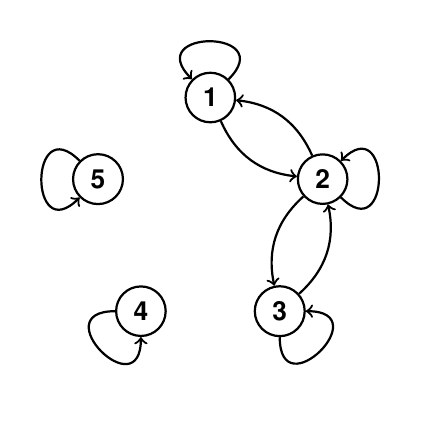
\begin{tikzpicture}[baseline, ->, thick, main node/.style={circle,draw,font=\sffamily\bfseries}]
	    \foreach \x in {1,2,3,4,5}
	        \node[main node](\x) at (162-72*\x:1.5cm) {\x};
        \draw (1) edge[loop, looseness=5] (1);
        \draw (2) to [out = -45, in = 45, looseness = 5] (2);
        \draw (3) to [out=270, in=0, looseness = 5] (3);
        \draw (4) to [out=180, in=270, looseness = 5] (4);
        \draw (5) to [out=135, in = 225, looseness = 5] (5);
        \draw (1) to [bend right] (2);
        \draw (2) to [bend right] (1);
        \draw (2) to [bend right] (3);
        \draw (3) to [bend right] (2);
        \end{tikzpicture} \hfill

\begin{enumerate}
    \item Is R reflexive? Is R symmetric? Is R transitive? (For this problem short Yes/No answers are acceptable.) 
    \item Add the minimum number of directed edges necessary to make the relation an equivalence relation.
    \item For the equivalence relation in part b, identify all the equivalence classes. 
\end{enumerate}

\item 
\begin{enumerate} 
\item (\textbf{C1, C3}) There are 24 students in our class, and we'd like to split everyone up into six groups of exactly 4. How many ways can we do this?\\
Carefully explain why the counting strategy you used is correct.


\item What if we're naming each of the six groups?\\
Carefully explain why the counting strategy you used is correct.

\end{enumerate}

\item (\textbf{P3}) Construct a \textbf{combinatorial} proof of the following binomial identity: 
\[\binom{n}{k} = \binom{n}{n-k}\]
(\textbf{Note:} A purely algebraic proof won't count here.)


\item (\textbf{C1, C2}) Suppose you have ten identical green balls.

\begin{enumerate}
    \item How many ways could these balls be distributed to four people? 
    \item How many ways could these balls be distributed to four people if everyone gets at least one? 
    \item How many ways could these balls be distributed to four people if nobody gets more than two balls?
\end{enumerate}


\item (\textbf{S2}) \textbf{NOTE: I think this problem is wrong!!!} Consider the following Venn diagrams and set descriptions:

W. 
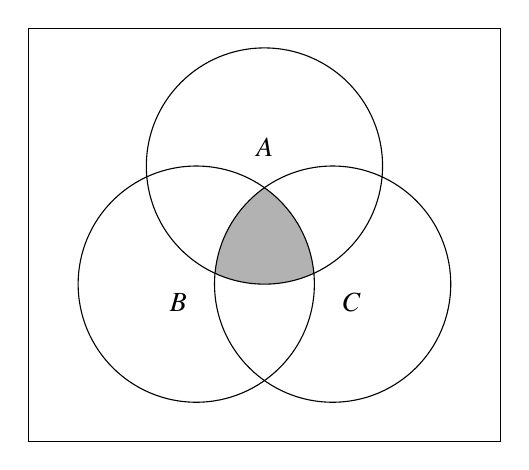
\begin{tikzpicture}
\begin{scope}
    \clip \firstcircle;
    \clip \secondcircle;
    \fill[lightgray] \thirdcircle;
\end{scope}
\draw \firstcircle node[text=black,above] {$A$};
\draw \secondcircle node [text=black,below left] {$B$};
\draw \thirdcircle node [text=black,below right] {$C$};
\draw \universer;
\end{tikzpicture}
\hfill
X. 
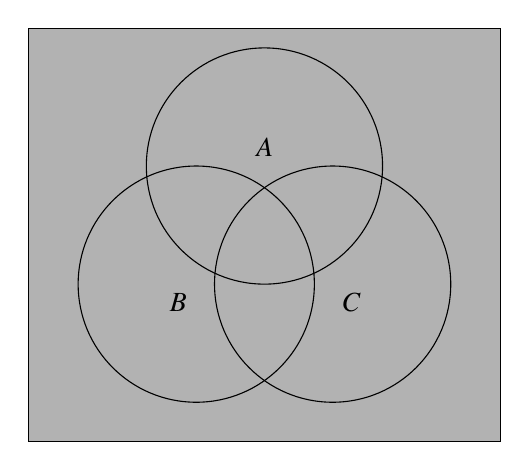
\begin{tikzpicture}
\fill[lightgray] \universer;
\draw \firstcircle node[text=black,above] {$A$};
\draw \secondcircle node [text=black,below left] {$B$};
\draw \thirdcircle node [text=black,below right] {$C$};
\draw \universer;
\end{tikzpicture}
\hfill\, % This is a ridiculous hack.

\hfill
Y.
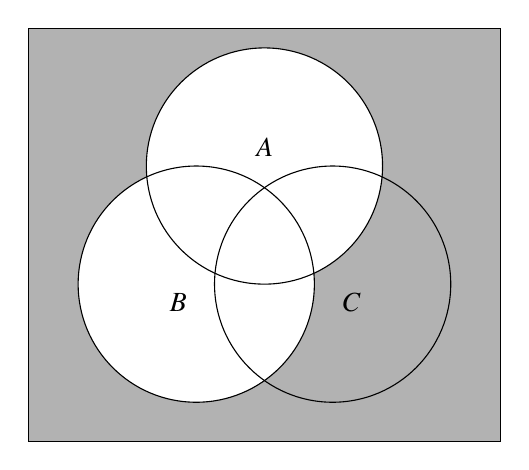
\begin{tikzpicture}
\begin{scope}[even odd rule]
    \clip \secondcircle \universer;
    \clip \firstcircle \universer;
    \fill[lightgray] \universer;
\end{scope}
\draw \firstcircle node[text=black,above] {$A$};
\draw \secondcircle node [text=black,below left] {$B$};
\draw \thirdcircle node [text=black,below right] {$C$};
\draw \universer;
\end{tikzpicture}
\hfill
Z. 
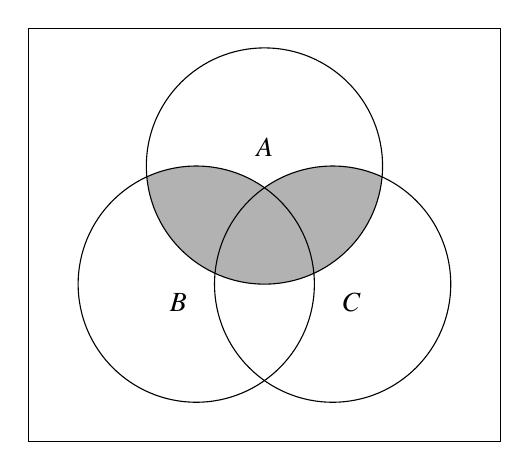
\begin{tikzpicture}
\begin{scope} % I genuinely have no idea why this works.
    \clip \secondcircle \thirdcircle;
    \fill[lightgray] \firstcircle;
\end{scope}
\draw \firstcircle node[text=black,above] {$A$};
\draw \secondcircle node [text=black,below left] {$B$};
\draw \thirdcircle node [text=black,below right] {$C$};
\draw \universer;
\end{tikzpicture}

i. $(\overline{A}) \cup (\overline{B})$
\hfill
ii. $\overline{(A \cup B)}$
\hfill
iii. $(A\cap B) \cup (A \cap C)$
\hfill
iv. $A\cap (B\cup A) \cap C$

\begin{enumerate}[(a)]
    \item Match the four Venn diagrams with the four set descriptions. Explain any Venn diagrams or sets that do not match. Carefully explain all of your choices.
    
   
    \item Explain why it's important to carefully use parentheses when writing set descriptions.
    
\end{enumerate}

\item Consider the Venn diagram matching task above.
\begin{enumerate}
    \item (\textbf{C1, C3}) How many total possible ways are there to match four Venn diagrams each to exactly one of four outcomes? Carefully explain why the counting strategy you used is correct.
    
    
    \item (\textbf{C2, C3}) If there is only one correct match for each Venn diagram, how many answers are \textbf{completely} incorrect -- that is, contain \textbf{no} correct matches? Carefully explain your solution.
    
\end{enumerate}

\item (\textbf{L2}) We keep saying that the negation of an implication $(P \to Q)$ is $(P \land \lnot Q)$.
\begin{enumerate}
    \item Write a truth table to show that this is correct.
    
    \item Carefully explain \textbf{why} your truth table shows that we're right.
    
\end{enumerate}

\pagebreak

\section*{MATH210 - Chapter 1 Quiz - Take-home portion}

\item (\textbf{S1}) Write the following sets in set-builder notation:

\begin{enumerate}
    \item $\{1, 4, 9, 16, 25, 36, ... \}$ \\
    \item $\{1, 4, 7, 10, 13, 16, ... \}$ \\
\end{enumerate}

\item (\textbf{P1}) Prove that an even integer minus an odd integer is an odd integer.

(\textbf{Note:} Our usual definitions of even and odd extend to the integers pretty naturally. For instance, $-3$ is also odd, and $-4$ is also even.)


\item
\textbf{(L3, S4)} In analyzing relations on a set we have studied the reflexive, symmetric, and transitive properties but there are other interesting and important properties. One of them is the antisymmetric property. Here is the definition:

Given relation R on set A, R is \textbf{antisymmetric} if and only if 

		\[\forall x \in A\ \forall y \in A, (xRy \land yRx) \rightarrow x = y \]

\begin{enumerate}
    \item Write an \textbf{equivalent} definition of antisymmetric in logical symbols using the contrapositive of the original definition. \\
	\item Write the \textbf{negation} of this definition in logical symbols. Simplify as much as possible. \\
	\item Draw two directed graphs for different relations on the set $A=\{w,x,y,z\}$, one that \textbf{IS} antisymmetric and one that is \textbf{NOT} antisymmetric.
\end{enumerate}

\item 
\textbf{(P5)}
Consider the following theorem: 

\begin{center} For all natural numbers $n$, if $n^{2}$ is even then $n$ is even. 
\end{center}

What follows is a supposed proof. Your job is to critique the proof by explaining what is wrong with it and by supplying a correct proof. Check it out:

    \begin{proof} Consider any $n \in \mathbb{N}$. 
    \begin{quote} 
    Assume that $n^{2}$ is even. \\  
    By definition, $n^{2} = 2k$ for some $k \in \mathbb{N}$.  \\
    Taking square roots on both sides,  $\sqrt{n^{2}}=\sqrt{2k}$. \\   
    Simplifying, $n=\sqrt{2k}$.   \\ 
    Multiplying by $2$ top and bottom inside the square root, $n=\sqrt{\frac{2\cdot 2k}{2}}$.   \\
    So, $n=\sqrt{\frac{4\cdot k}{2}}$. \\   
    Pulling $4$ out of the square root, $n=2\cdot\sqrt{\frac{k}{2}}$.  \\
    Let $m=\sqrt{\frac{k}{2}}$. \\ 
    Thus, $n=2m$.  \\
    Therefore, $n$ is an even number.  \\
    So, our theorem is proved!?
    \end{quote}
    \end{proof}
\end{enumerate}
\end{document}
